\documentclass[10pt]{extarticle}

\usepackage[margin=1.8cm]{geometry}
\usepackage{amsmath,amssymb}
\usepackage{enumitem}
\usepackage{graphicx}
\usepackage{listings}
\usepackage{xcolor}
\usepackage[
  colorlinks=true,
  linkcolor=blue!50!black,
  urlcolor=blue!60!black
]{hyperref}

\setlist{itemsep=2pt,topsep=4pt}
\lstset{
  basicstyle=\ttfamily\small,
  keywordstyle=\color{blue!60!black}\bfseries,
  commentstyle=\color{green!40!black}\itshape,
  frame=single,
  numbers=left,
  numberstyle=\scriptsize\color{black!55},
  numbersep=8pt,
  showstringspaces=false,
  columns=fullflexible,
  keepspaces=true
}

\title{Tanaka Certificates: Weekly Research Report}
\author{Filip Morawiec}
\date{6 July 2026}

\begin{document}

\maketitle

\begin{abstract}
This week I contributed by implementing a multidimensional verifier for ReLU neural 
networks (with last layer being piecewise quadratic to ensure completeness) and 
beginning to prove its correctness. 
After meeting with Greg, he recommended that I should focus on proving the correctness 
of the ReLU NN region discovery algorithm and algebraically working through an example 
2D SDE verification, which I initially did and present here.
I also worked on training a certificate for this problem - following the techniques used 
by Greg in his previous paper -  but I failed to satisfy all the constraints a 
certificate should have.
\end{abstract}

\tableofcontents
\newpage

\section{Multidimensional verifier}

\subsection{Problem setup}

Consider a multi-dimensional stochastic differential equation
\begin{equation}
  dX_t=f(X_t)\,dt+g(X_t)\,dW_t
  \label{eq:sde}
\end{equation}
on a domain $D \subset \mathbb{R}^d$, where
$f:\mathbb{R}^d\to\mathbb{R}^d$ is the drift,
$g:\mathbb{R}^d\to\mathbb{R}^{d\times m}$ is the diffusion, and $W_t$
is an $m$-dimensional Brownian motion.  Write
$a(x)=g(x)g(x)^\top$ for the diffusion covariance.  For a
reach--avoid problem, let $X_0\subseteq D$ be the
initial set, $X_u\subseteq D$ the unsafe set, and $X_\tau\subseteq D$ the target.
We seek a certificate $V$ and constants $\alpha<\beta$ and $\varepsilon>0$
such that
\begin{enumerate}
  \item boundary condition holds: 
  \begin{equation}
    \label{eq:boundary-conditions}
    \sup_{x\in X_0}V(x)\leq\alpha \qquad\text{and}\qquad
    \inf_{x\in X_u}V(x)\geq\beta
  \end{equation}
  \item generator condition holds: 
  \begin{equation}
    \label{eq:generator-conditions}
    \mathcal LV(x)\leq-\varepsilon \qquad\text{for }x\in\{V\leq\beta\}\setminus X_\tau,
  \end{equation}
\end{enumerate}
where, at smooth points,
\begin{equation}
  \mathcal LV(x)
  =\nabla V(x)\cdot f(x)
  +\frac12\operatorname{tr}\!\left(a(x)\nabla^2V(x)\right).
  \label{eq:generator}
\end{equation}

Following the piecewise-quadratic setup, suppose that a compact verification
region $K\subseteq D$ is partitioned into finitely many polyhedral cells,
\[
  K=\bigcup_{i=1}^N K_i,
\]
and that $V$ is continuous across their interfaces and quadratic on each cell:
\begin{equation}
  V(x)=V_i(x)
  =c_i+p_i^\top x+\frac12x^\top Q_i x,
  \qquad x\in K_i, \qquad Q_i=Q_i^\top.
  \label{eq:pwq-cell}
\end{equation}
Consequently, inside $K_i$,
\begin{equation}
  \mathcal LV_i(x)
  =(p_i+Q_i x)\cdot f(x)
  +\frac12\operatorname{tr}\!\left(a(x)Q_i\right).
  \label{eq:pwq-generator}
\end{equation}
Besides the interior generator condition, the multidimensional
It\^o--Tanaka formula introduces a surface-local-time term on cell interfaces.
For every shared face $F$ between $K_i$ and $K_j$, with unit normal
$n_{i\to j,F}$ pointing from $K_i$ to $K_j$, this contribution is
nonpositive when
\begin{equation}
  \left(\nabla V_j(x)-\nabla V_i(x)\right)\cdot n_{i\to j,F}
  =\left(p_j-p_i+(Q_j-Q_i)x\right)\cdot n_{i\to j,F}
  \leq 0,
  \qquad x\in F.
  \label{eq:interface-condition}
\end{equation}
Together with square-integrability of the stochastic integral, continuity,
the cellwise generator condition, and this interface condition ensure that
$V(X_t)$ is a supermartingale up to the first exit time from $K$.

The process is stopped after reaching the target or unsafe set: once the
reach--avoid property has been achieved or violated, its later trajectory is
irrelevant.

\begin{quote} 
  \textbf{Remark}. \label{remark:piecewise-quadratic} We model a certificate $V$ as:
  \begin{align}
    V(x) &= \sum_{k=1}^m \lambda_k\phi(z_k(x))+c, \\
    z(x) &= \texttt{NN}(x)
      = W_L\texttt{ReLU}(\ldots\texttt{ReLU}(W_1x+b_1)\ldots)+b_L, \\
    \phi &= \texttt{PiecewiseQuadratic1D}.
  \end{align}
  This way, because we include a piecewise quadratic function $\phi$ in the last layer, 
  we cover a certain failure case related to the curvature term $V''(x)$ in the 
  generator condition \eqref{eq:generator-conditions}.    
\end{quote}


\section{1D ReLU NN region discovery}

Consider the following Algorithm~\ref{alg:discover-1d-cells}  which discovers the linear cells of a one-dimensional ReLU network.

\begin{lstlisting}[
  language=Python,
  caption={Discover one-dimensional linear cells of a ReLU network},
  label={alg:discover-1d-cells}
]
def discover_cells(layers):
    """
    The network has a one-dimensional input and a one-dimensional output, but hidden
    layers can be multi-dimensional:
    >>> layers[i] = (W_i, b_i)
    >>> W_i.shape = (n_{i+1}, n_i)
    >>> b_i.shape = (n_{i+1},)    
    """

    # A cell is (lower, upper, slope, intercept).
    cells = [(-inf, inf, [1], [0])]

    for W, b in layers:
        new_cells = []
        for lower, upper, slope, intercept in cells:
            # key observation: in a cell C_prev(l, u, slope, intercept), we have 
            #   z_prev = slope @ x + intercept, so the linear function 
            # in the current cell C(?, ?, alpha, beta) will be
            #   z = W @ z_prev + b = (W @ slope) @ x + (W @ intercept + b)
            alpha = W @ slope
            beta = W @ intercept + b

            roots = {
                -beta[j] / alpha[j]
                for j in range(len(beta))
                if alpha[j] != 0
                and lower < -beta[j] / alpha[j] < upper
            }
            boundaries = [lower, *sorted(roots), upper]

            for left, right in consecutive_pairs(boundaries):
                x = choose_point(left, right)
                active = alpha @ x + beta > 0 # list of booleans
                new_slope = where(active, alpha, 0)
                new_intercept = where(active, beta, 0)
                new_cells.append(
                    (left, right, new_slope, new_intercept)
                )

        cells = new_cells

    return cells
\end{lstlisting}

It discovers the linear cells of a one-dimensional ReLU network, with:
\begin{align}
  \texttt{NN}(x) &= W_L\texttt{ReLU}(\ldots\texttt{ReLU}(W_1x+b_1)\ldots)+b_L.
\end{align}

To prove the correctness algorithms, the key step is to show, given a linear cell of the
network up to layer \(m-1\), how to discover the linear cells of the network up to layer \(m\).

As a precondition, we already have a linear cell of the network when we begin: 
$\texttt{C(-$\infty$, $\infty$, [1], [0])}$ represents the entire real line, with slope [1] and intercept [0].

Now, assume at layer \(m-1\) we have a linear cell \(\texttt{C(l, u, slope, intercept)}\) which is 
correctly discovered.  Then, at layer \(m\), as shown in the code comment, we have a linear function:
\begin{equation}
  z = W \texttt{@} \ z_{m-1} + b = (W \texttt{@} \ \text{slope}) \texttt{@} x + (W \texttt{@} \ \text{intercept} + b)
\end{equation}

Since $z$ is a list of $n_m$ elements, we have to check when $z_j = 0$ for each $j=1,\ldots,n_m$.  
This gives us the new potential breakpoints.

Now, to determine how the resulting cells are formed, we can take a point within each interval 
$(\texttt{breakpoint}_i, \texttt{breakpoint}_{i+1})$ and check whether the resulting neuron 
would be active. This yields the new slope and intercept for that cell.

\vspace{1em}
\hrule 
\vspace{1em}


Note that in the actual implementation, the last layer is piecewise quadratic as noted in
Remark \ref{remark:piecewise-quadratic}, but the reasoning is similar. We just further
have to break up the cells based on the breakpoints of the piecewise quadratic function.

\section{Multi-dimensional ReLU NN region discovery}

We now extend Algorithm~\ref{alg:discover-1d-cells} to the multi-dimensional input case.
The main difference is that the cells are no longer intervals, but convex polyhedra.

Consider a ReLU network
\begin{align}
\texttt{NN}(x) &= W_L\texttt{ReLU}(\ldots\texttt{ReLU}(W_1x+b_1)\ldots)+b_L,
\end{align}
where now $x \in \mathbb{R}^{d}$.  As before, hidden layers can be multi-dimensional:
\[
W_i \in \mathbb{R}^{n_{i+1}\times n_i},
\qquad
b_i \in \mathbb{R}^{n_{i+1}}.
\]

In the one-dimensional case, a cell was represented by
\[
\texttt{C(l, u, slope, intercept)}.
\]
In the multi-dimensional case, we instead represent a cell by
\[
\texttt{C(A, c, slope, intercept)},
\]
where
\[
A x \leq c
\]
describes the current polyhedral region, and on this region we have
\[
z_{m-1} = \text{slope} \ x + \text{intercept}.
\]
Here
\[
\text{slope} \in \mathbb{R}^{n_{m-1}\times d},
\qquad
\text{intercept} \in \mathbb{R}^{n_{m-1}}.
\]

As a precondition, we already have a linear cell of the network when we begin:
\[
\texttt{C([], [], I, 0)}
\]
represents the entire space $\mathbb{R}^d$, with slope $I$ and intercept $0$.

Now, assume at layer $m-1$ we have a linear cell
\[
\texttt{C(A, c, slope, intercept)}
\]
which is correctly discovered.  Then, at layer $m$, we again have a linear function:
\begin{equation}
z = W \texttt{@} \ z_{m-1} + b
= (W \texttt{@} \ \text{slope}) \texttt{@} x
+ (W \texttt{@} \ \text{intercept} + b).
\end{equation}
Therefore define
\begin{align}
\alpha &= W \texttt{@} \ \text{slope}, \\
\beta  &= W \texttt{@} \ \text{intercept} + b.
\end{align}
Then, inside the current cell, every pre-activation is of the form
\begin{equation}
z_j = \alpha_j x + \beta_j,
\end{equation}
where $\alpha_j$ is the $j$-th row of $\alpha$.

In the one-dimensional case, the possible new boundaries were points satisfying
\[
\alpha_j x + \beta_j = 0.
\]
In the multi-dimensional case, the possible new boundaries are hyperplanes:
\begin{equation}
\alpha_j x + \beta_j = 0,
\qquad j=1,\ldots,n_m.
\end{equation}

Each such hyperplane splits the current polyhedral cell into two possible pieces:
\begin{align}
\alpha_j x + \beta_j &\geq 0,
&&\text{where neuron } j \text{ is active}, \\
\alpha_j x + \beta_j &\leq 0,
&&\text{where neuron } j \text{ is inactive}.
\end{align}

Thus, instead of sorting roots on the real line, we refine the current region by intersecting it
with all possible activation constraints.  Equivalently, for each activation pattern
\[
s \in \{0,1\}^{n_m},
\]
we construct the candidate region
\begin{equation}
R_s =
\left\{
x :
A x \leq c,
\quad
\alpha_j x + \beta_j \geq 0 \ \text{if } s_j=1,
\quad
\alpha_j x + \beta_j \leq 0 \ \text{if } s_j=0
\right\}.
\end{equation}

If $R_s$ is non-empty, then it is a new linear cell.  On this cell, the ReLU activation is fixed,
so we get
\begin{align}
\texttt{new\_slope}
&= \texttt{where}(s, \alpha, 0), \\
\texttt{new\_intercept}
&= \texttt{where}(s, \beta, 0).
\end{align}
This is the exact multi-dimensional analogue of the one-dimensional update.

\newpage

The corresponding algorithm is:

\begin{lstlisting}[
language=Python,
caption={Discover multi-dimensional linear regions of a ReLU network},
label={alg:discover-multidim-cells}
]
def discover_regions(layers, d):
  """
  The network has a d-dimensional input. Hidden layers can be multi-dimensional:
  >>> layers[i] = (W_i, b_i)
  >>> W_i.shape = (n_{i+1}, n_i)
  >>> b_i.shape = (n_{i+1},)
  """

  # A cell is (A, c, slope, intercept), where
  #   A @ x <= c
  # A.shape = (num_constraints, d)
  # slope.shape = (num_constraints, d)
  # and inside this region
  #   z = slope @ x + intercept.
  cells = [([], [], I_d, 0)]

  for W, b in layers:
      new_cells = []
      for A, c, slope, intercept in cells:
          # key observation: in a cell C(A, c, slope, intercept), we have
          #   z_prev = slope @ x + intercept, so the linear function
          # in the current cell C(?, ?, alpha, beta) will be
          #   z = W @ z_prev + b = (W @ slope) @ x + (W @ intercept + b)
          alpha = W @ slope
          beta = W @ intercept + b

          for active in all_boolean_patterns(len(beta)):
              A_new = list(A)
              c_new = list(c)

              for j in range(len(beta)):
                  if active[j]:
                      # alpha[j] @ x + beta[j] >= 0
                      # equivalently: -alpha[j] @ x <= beta[j]
                      A_new.append(-alpha[j])
                      c_new.append(beta[j])
                  else:
                      # alpha[j] @ x + beta[j] <= 0
                      # equivalently: alpha[j] @ x <= -beta[j]
                      A_new.append(alpha[j])
                      c_new.append(-beta[j])

              if is_nonempty_polyhedron(A_new, c_new):
                  new_slope = where(active, alpha, 0)
                  new_intercept = where(active, beta, 0)
                  new_cells.append(
                      (A_new, c_new, new_slope, new_intercept)
                  )

      cells = new_cells

  return cells
\end{lstlisting}

To prove the correctness of the algorithm, the key step is again to show, given a linear cell of
the network up to layer $m-1$, how to discover the linear cells of the network up to layer $m$.

Assume that at layer $m-1$ we have correctly discovered a cell
\[
\texttt{C(A, c, slope, intercept)}.
\]
By correctness of this cell, for all $x$ satisfying $A x \leq c$, we have
\[
z_{m-1} = \text{slope} \ x + \text{intercept}.
\]
After applying the affine map of layer $m$, we obtain
\[
z = Wz_{m-1}+b
= (W \texttt{@} \ \text{slope})x
+ (W \texttt{@} \ \text{intercept}+b)
= \alpha x + \beta.
\]
Therefore, inside the current cell, the sign of each neuron is determined by the affine inequality
\[
\alpha_j x + \beta_j \gtreqless 0.
\]

The ReLU is linear exactly on regions where these signs are fixed.  Hence, the current cell must
be split according to all possible choices of signs of
\[
\alpha_1 x + \beta_1,\ldots,\alpha_{n_m}x+\beta_{n_m}.
\]
For a fixed activation pattern $s$, the region $R_s$ is precisely the set of points in the old
cell which realize that activation pattern.  If this region is empty, then that pattern never
occurs in the old cell and should be discarded.  If it is non-empty, then the ReLU output on this
region is
\[
\texttt{ReLU}(z)_j =
\begin{cases}
\alpha_j x + \beta_j, & s_j=1, \\
0, & s_j=0.
\end{cases}
\]
Thus, on $R_s$, the new representation is exactly
\begin{align}
\texttt{new\_slope}
&= \texttt{where}(s, \alpha, 0), \\
\texttt{new\_intercept}
&= \texttt{where}(s, \beta, 0).
\end{align}

Therefore every non-empty region generated by the algorithm is a correct linear cell for the
network up to layer $m$. Conversely, any true linear cell of the network up to layer $m$ must
lie inside some previously discovered cell at layer $m-1$, and must have a fixed activation
pattern at layer $m$. Hence it is contained in one of the non-empty regions $R_s$ constructed
above. This proves that the algorithm discovers exactly the linear cells of the network layer by
layer.

\vspace{1em}
\hrule
\vspace{1em}

Note that, just as in the one-dimensional case, if the last layer is piecewise quadratic as noted
in Remark \ref{remark:piecewise-quadratic}, the same reasoning applies.  The only difference is
that instead of further splitting intervals by the breakpoints of the piecewise quadratic
function, we further split polyhedral cells by the hypersurfaces on which the corresponding
piecewise quadratic expression changes.


\section{2D SDE verification example}

\newpage

\section{Certificate training}

\begin{figure}[h]
  \centering
  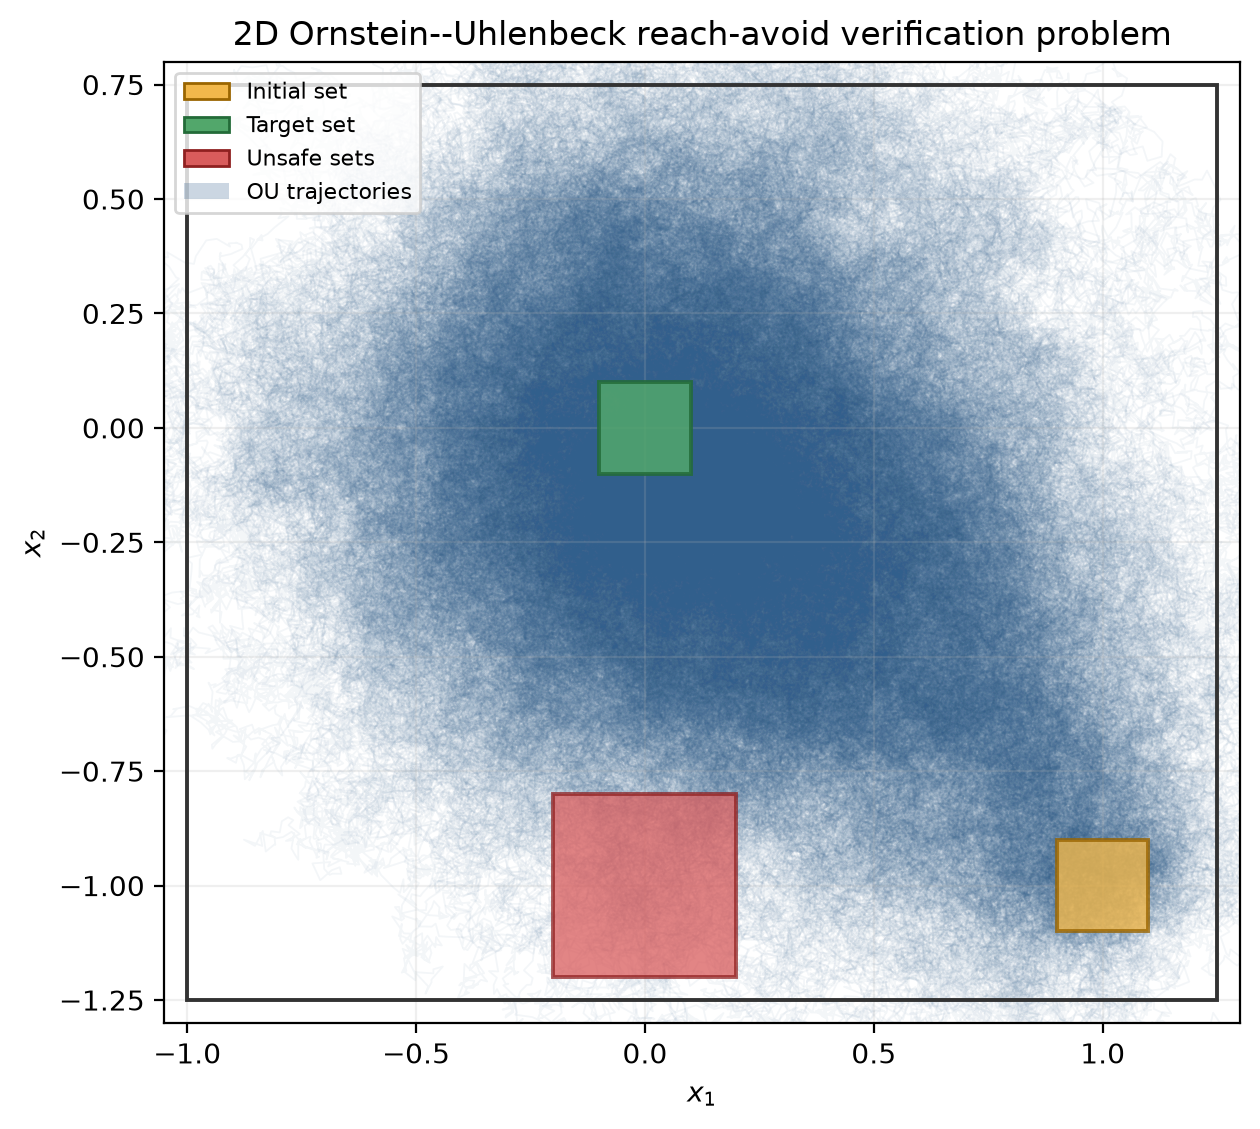
\includegraphics[width=0.425\textwidth]{img/verifier_pwq_2d_ornstein_uhlenbeck.png}
  \caption{Verification of a piecewise-quadratic certificate for the
  two-dimensional Ornstein--Uhlenbeck process.}
  \label{fig:verifier-pwq-2d-ou}
\end{figure}

Before Greg gave feedback on my work, I was working on training a piecewise-quadratic certificate
for a problem of an Urnstein--Uhlenbeck process in 2D, as seen on Figure~\ref{fig:verifier-pwq-2d-ou}.  

I was training the certificate with the losses:
\begin{enumerate}
  \item \textbf{Boundary loss.}  On sampled points from the initial and unsafe
  sets, including all corners of their hyperrectangles, I penalized
  \(
    \max\{V(x)- (\alpha-\delta),0\}
  \)
  for $x\in X_0$ and
  \(
    \max\{(\beta+\delta)-V(x),0\}
  \)
  for $x\in X_u$, where the constraint margin was $\delta=0.1$.

  \item \textbf{Generator loss.}  For sampled domain points outside the target,
  I penalized the cheaper of the two violations
  \[
    \max\{\mathcal{L}V(x)+\varepsilon+\delta_{\mathcal L},0\}
    \quad\text{and}\quad
    \max\{\beta+\delta-V(x),0\},
  \]
  with generator margin $\delta_{\mathcal L}=0.02$.  This reflects the
  disjunctive condition that either $x\notin\{V\leq\beta\}$ or the generator
  must be sufficiently negative.  This loss was enabled after 50 epochs of
  boundary pretraining.

  \item \textbf{Concavity loss.}  For sampled pairs $x,y$ from the same
  hyperrectangle, I penalized violations of midpoint concavity,
  \[
    \max\left\{\frac{V(x)+V(y)}{2}
      -V\left(\frac{x+y}{2}\right),0\right\}.
  \]

  \item \textbf{Regularization.}  I added a small mean-squared parameter
  penalty to discourage unnecessarily large network weights.
\end{enumerate}

I verified it with an approximate verifier (that samples points instead of checking the entire region)
and it found some violations of the certificate conditions, as seen on Figure~\ref{fig:trained-pwq-certificate-comparison}.  

\begin{figure}[h]
  \centering
  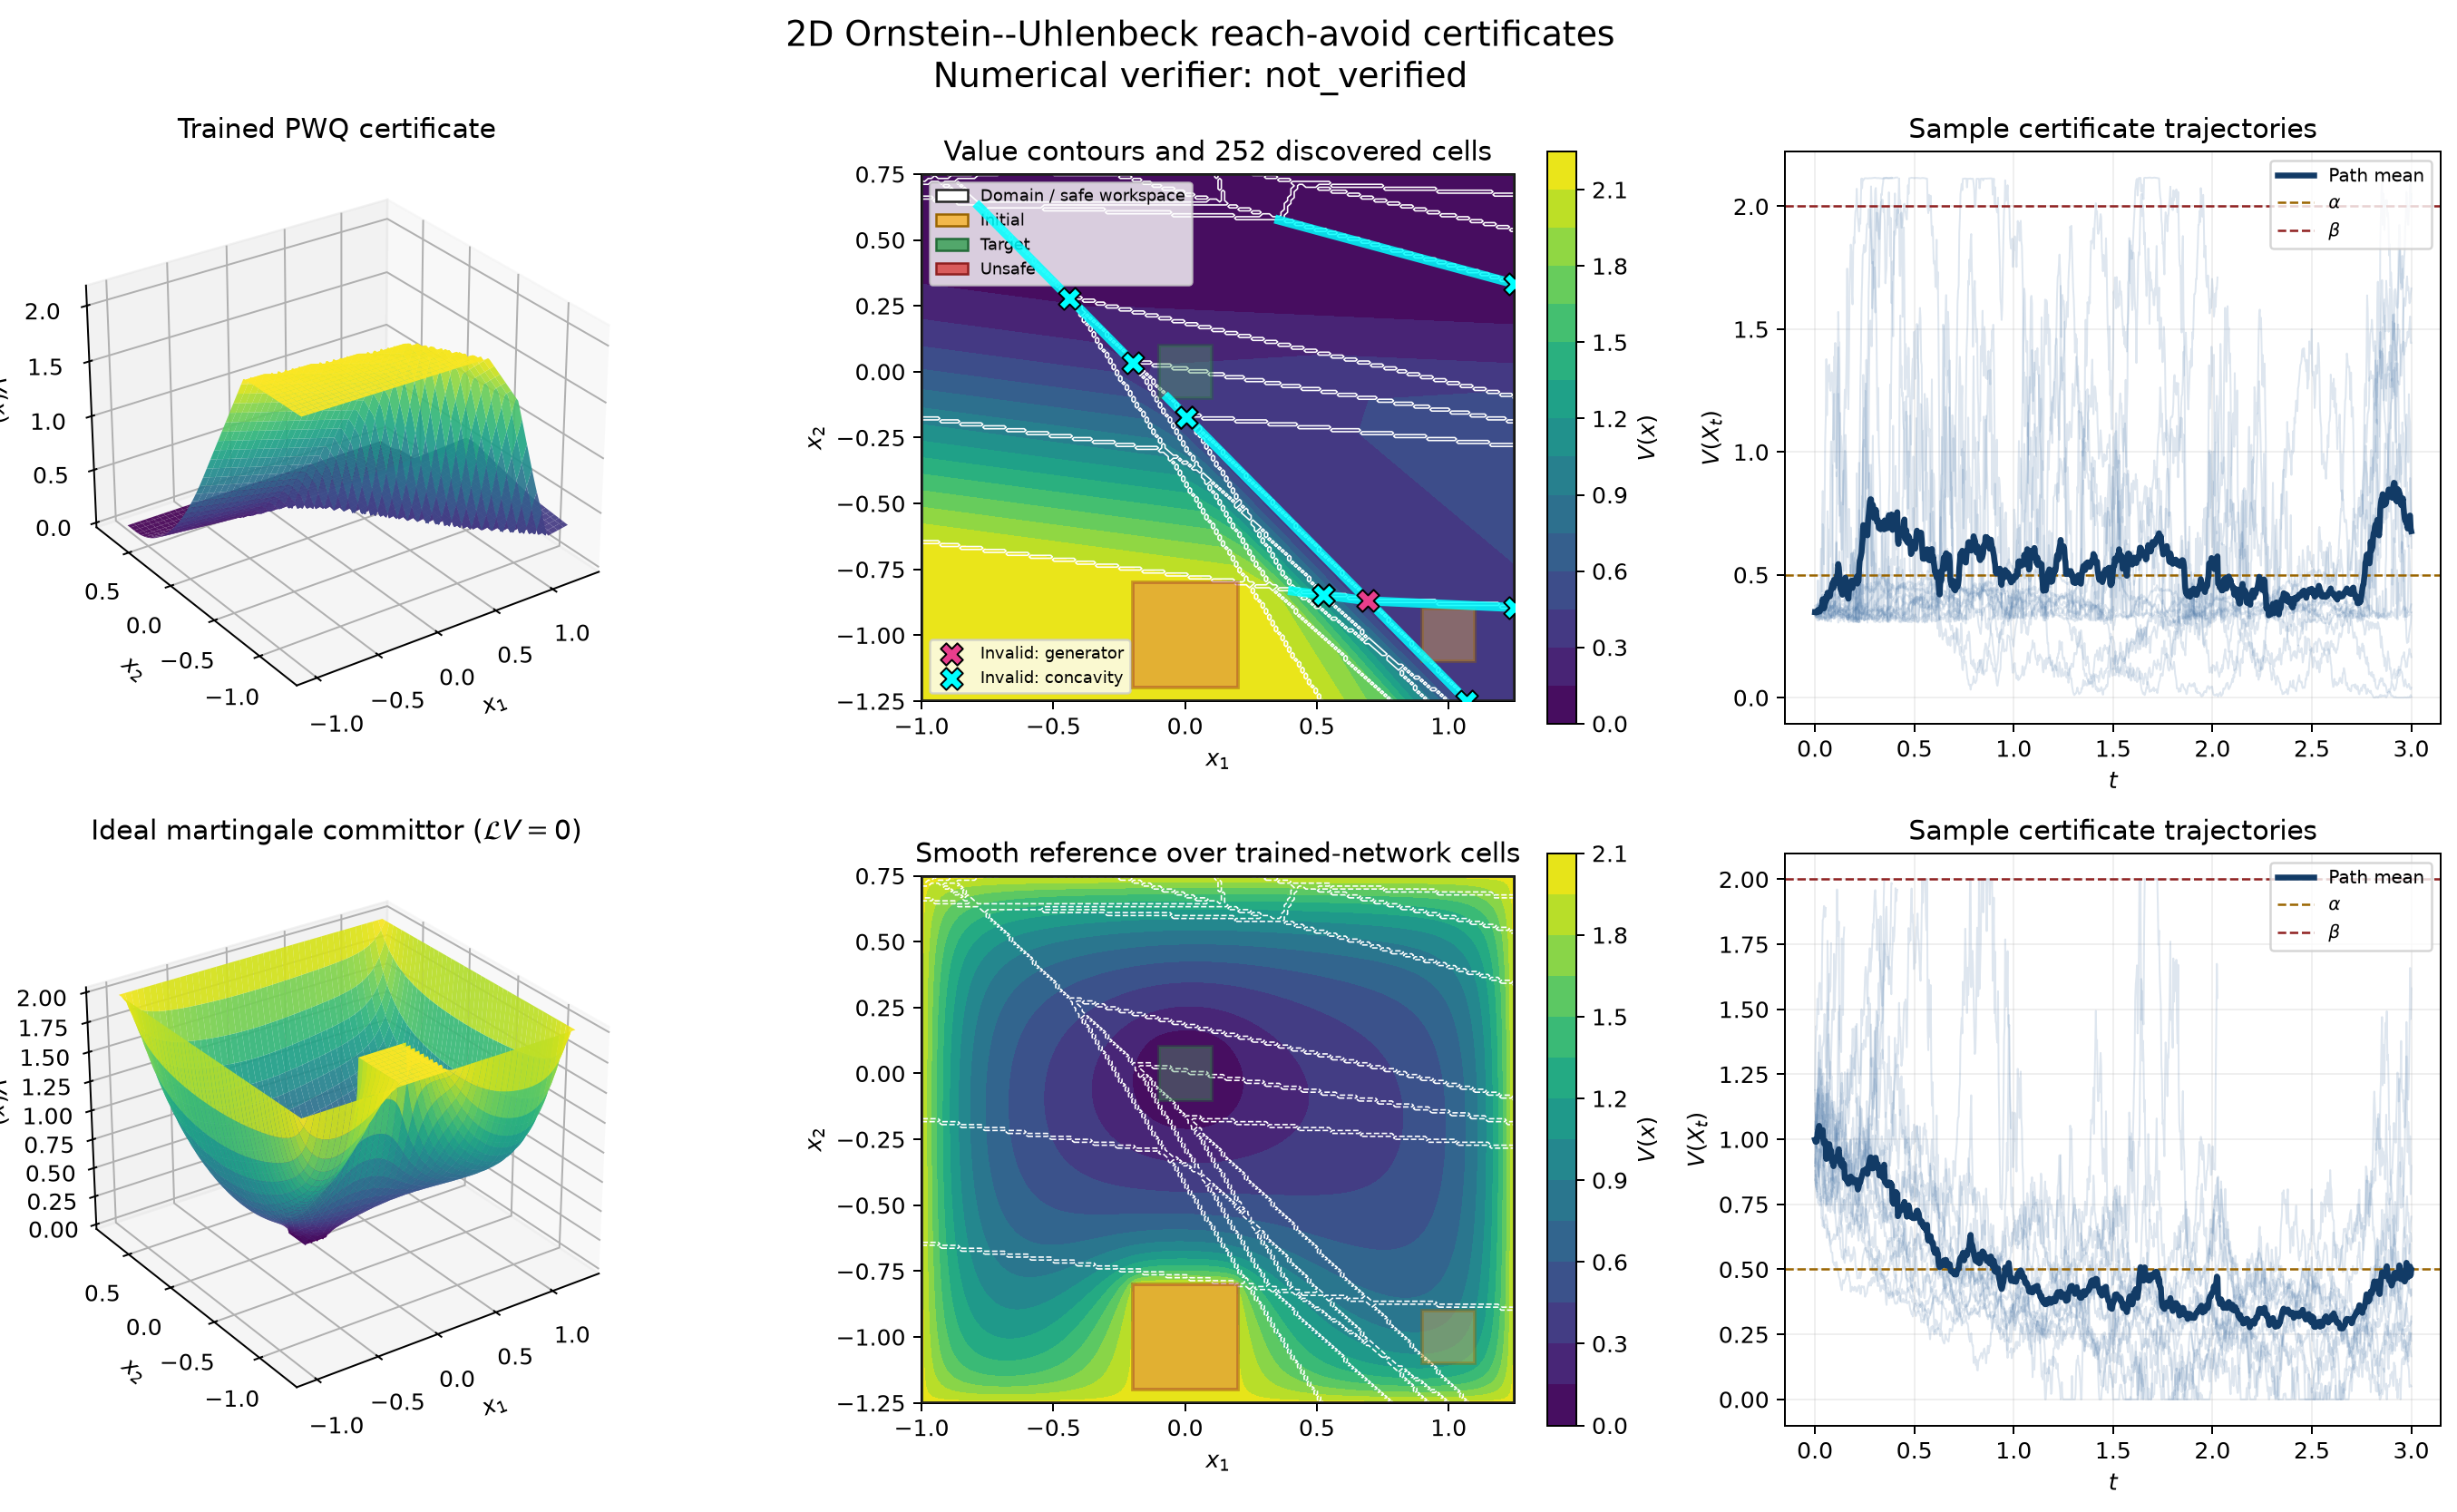
\includegraphics[width=0.85\textwidth]{img/certificate_comparison.png}
  \caption{Comparison of the trained piecewise-quadratic certificate.}
  \label{fig:trained-pwq-certificate-comparison}
\end{figure}


\end{document}
